\section{Related \& Future Work} \label{sec:relatedwork}
\textbf{One Big Switch:} Kang et. al~\cite{oneswitch} tackle a 
similar problem of flow policy
enforcement. However, their end-point policies deal with simple
reachability. Their rule placement algorithm takes the path of the
flow in the network (called the routing policy) as an input. %  and place rules
% on this path to enforce the endpoint policy and taking in
% consideration switch table constraints
% Our solution can support enforcement of policies which
% require different routing policies.
Zhang et. al~\cite{distfirewall} build on the "one big switch"  
abstraction~\cite{oneswitch} to optimize for the specific case of
distributed firewall policy enforcement using ILP.  PGA~\cite{pga} provides
a graph-level abstraction for specifying network policies like ACLs and
middlebox service chaining. However, PGA abstracts the underlying
network as "one big switch" and cannot be used to compose policies like
tenant isolation or traffic engineering.
\begin{figure}[t]
	\centering
	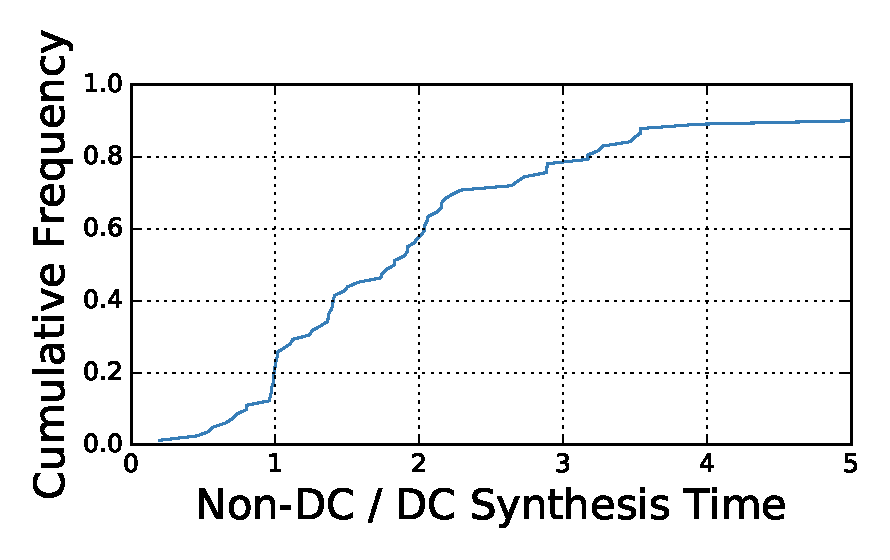
\includegraphics[width=0.7\columnwidth]{figures/dcSynthesis.eps}
	\compactcaption{CDF for speedup achieved by divide-and-conquer synthesis.}
	\label{fig:dcsyn-cdf}
\end{figure}

 \noindent {\bf Controller synthesis:}
 Program synthesis has
 seen limited applications to SDN controllers~\cite{netegg,decentralize}.
These systems synthesize the
 behavior of individual switches (e.g., learning switches or
 firewalls); furthermore, these techniques apply to networks
 operating in a reactive mode (where the first packet of a connection
 is processed by the controller to determine the actions to
 employ). Such switch-centric approaches are too constraining and
 cannot be applied to realize network-wide objectives considered 
 in \name.
 Synthesis has been also used for generating consistent network
 updates~\cite{updates, customconsistency}. But this problem is orthogonal to 
 policy enforcement.
 
\noindent {\bf Policy languages:}
The closest approaches to ours are Merlin~\cite{merlin},
NetGen~\cite{netgen} and NetKAT~\cite{netkat}.  
In Merlin, data planes that adhere to policies
expressed using regular expressions are synthesized by first
intersecting the topology with the regular expressions appearing in
the policies and then encoding reachability in the intersected graph
using mixed integer linear programming (ILP).
%Unlike \Name, 
Merlin supports minimum and maximum bandwidth guarantees.
In its current iteration, 
Merlin's encoding does not support isolation policies, but we believe
that it could be extended to support them.  
%We cannot evaluate the
%performance impact of this extension, however.  
A more prominent
difference arises with unordered waypoint policies: expressing a
policy including a waypoint set $W$ of size $k$ requires a regular
expression of size exponential in $k$ as all the possible permutations
of the elements of $W$ must be considered. This fact clearly 
impacts the performance of 
Merlin's compiler that would have to generate a mixed ILP with a
large number of variables.  In \Name, this is not the case as waypoints
can be encoded with polynomially many constraints.  While this does
not affect the theoretical complexity, our compiler does not incur
an a-priori exponential blow-up; it rather relies on the power
of SMT solvers to guide the search.  This is one of the main aspects
behind our decision of not using regular expressions to express
policies.  \Name uses a restricted form of regular expressions as 
tactics that leverage the network topology.  While in Merlin,
regular expressions \emph{increase} the number of constraints
generated by the compiler, tactics \emph{decrease}
the number of generated constraints, therefore speeding up the search.
To the best of our knowledge, this is the first use of constraints
that leverages the topology structure to simplify the search.

In NetGen, network updates that adhere to policies expressed using
regular expressions are synthesized using SMT solvers.  Given a
specification which mentions the packet classes, the old path, and the
new path, NetGen solves the network change problem using an SMT solver.
Due to the use of regular expressions NetGen also suffers the
limitations we just discussed for Merlin. Interestingly, NetGen uses
a specific encoding of regular expressions based on uninterpreted
functions that helps reduce the number of constraints. While this
encoding is fast when updating a single path, we do not see a way to
extend it to our global synthesis setting.  A crucial aspect of NetGen
is that in its problem formulation each path can be synthesized
independently and without affecting the other already synthesized
paths.  This is not the case when supporting isolation policies: if an
old path needs to be moved to satisfy a new policy (e.g., because a
link is under maintenance), re-synthesizing such a path can require
re-synthesizing other paths. 

NetKAT is a domain-specific language and logic for 
specifying and verifying network packet-processing functions
for SDN, based on Kleene algebra with tests (KAT). Semantically,
a NetKAT predicate and policy is a function that takes a packet
history and produces a set of (possibly empty) packet histories. 
NetKAT can be used to express certain network-wide policies like 
reachability, waypoints using regular expressions for describing the paths, 
and programs on virtual topologies; it uses
BDDs and symbolic automata to translate global programs to local
switch programs~\cite{netkatcompiler}. 
However, the NetKAT semantics
cannot be used to express policies based on hyperproperties
~\cite{hyperproperties}, i.e., 
the packet processing function requires multiple packet histories
as input. Traffic engineering or isolated paths are policies
based on hyperproperties. 
% \loris{we can have a small example of  this in appendix.}
\begin{figure}[t]
	\centering
	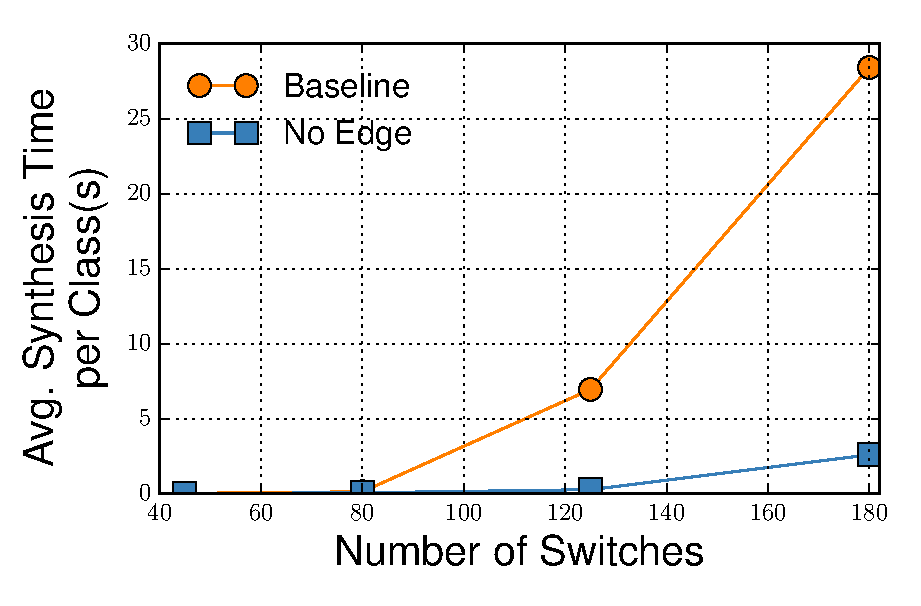
\includegraphics[width=0.65\columnwidth]{figures/linkTopology.eps}
	\compactcaption{Average synthesis time per packet class versus topology size for isolation workloads 
		with the ratio of packet classes to number of edge-aggregate links 0.25 and 10 low bandwidth links in the topology 
		have capacity policies.}
	\label{fig:link-capacity}
\end{figure}
% \noindent
% {\bf Synthesis for SDN:}
% Program synthesis has been actively applied in SDN for synthesizing the controller. Padon et. al in \cite{decentralize} try to synthesize
% local forwarding rules for a single switch based on a reactive
% forwarding policy.  NetEgg \cite{netegg} synthesizes the forwarding
% policy of a switch using examples of how the switch should function
% when it receives packets. These works deal with synthesis of
% forwarding behaviour of switches, and cannot be extended to satisfy
% network-wide policies.

% Write about PGA, NetGen, and efficient update synthesis.

\noindent
{\bf Future directions:}  
Fine-grained traffic engineering based on online demand/flow size estimation and 
rapid rerouting is also crucial for datacenter workloads, and extending \name's
TE policies to fine-grained timescales is subject of future work.
Also, the performance
of SMT solvers with optimization objectives is quite slow, and calls for 
domain-specific techniques to speed up the synthesis. Also, datacenter
networks are highly symmetrical, and this symmetry can be leveraged
to speed up synthesis (similar to the work of Plotkin et. al~\cite{symmetry} to
speed up network verification using symmetry). The main challenges of
using symmetry in synthesis is considering two aspects of symmetry: network
symmetry and policy symmetry. Also, our treatment of resilience synthesis
is preliminary and future work will be geared towards synthesizing resilient
forwarding planes incorporating capacity constraints and traffic engineering.
 
